%!TEX root = ../dokumentation.tex

\chapter{Softwaretechnik}

Dieses Kapitel enthält alle benötigten Software- und Hardware-Tools sowie die verwendeten Versionen.

\section{Softwarepakete}

Die Betreibssysteme auf denen gearbeitet wurde sind:

\begin{itemize}
  \item Windows 10 Enterprise 22H2
  \item macOS
\end{itemize}

\section{Entwicklungsumgebung}

Die folgenden Entwicklungsumgebungen, Erweiterungen und Tools wurden verwendet:

\begin{itemize}
  \item Visual Studio Code v.1.84.2
  \begin{itemize}
    \item Erweiterung Dart v3.78.0
    \item Erweiterung Flutter v3.78.0
  \end{itemize}
  \item Android Studio Giraffe | 2022.3.1 Patch 4
  \item Android SDK version 34.0.0
  \item Flutter v.3.16.0
  \item Visual Studio Community 2022 17.8.1
\end{itemize}


\section{Emulation}

Die App wurde sowohl im Simulator, als auch auf zwei physischen Endgeräten getestet.
Die verwendeten Geräte umfassen:

iOS:

\begin{itemize}
  \item Simulator: iPhone SE (3rd Generation), iOS 17.0
\end{itemize}

Die iOS-Simulation wurde mit dem SimulatorKit von Apple in der Version 15.0.1 (1015.2) ausgeführt.

Android:

\begin{itemize}
  \item Simulator: Pixel 3a, Api-Version 27, Android 8.1 (Oreo)
  \item Simulator: Pixel 3a, Api-Version 34, Android 14
  \item Simulator: Pixel 2, Api-Version 34, Android 14
\end{itemize}

Die Emulatoren haben folgende Eigenschaften und Einstellungen:

\begin{figure}[H]
    \centering
    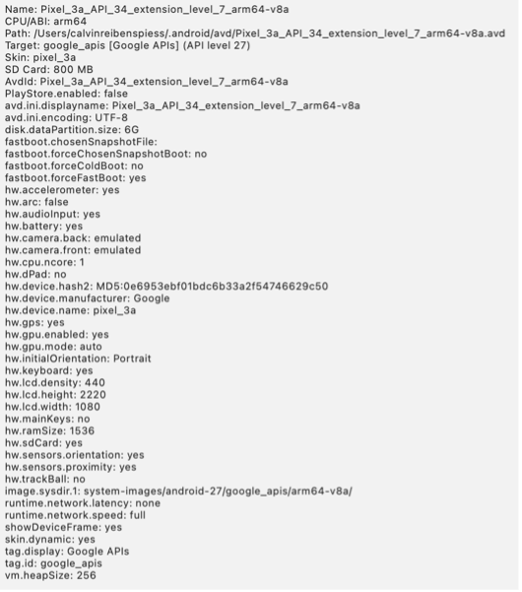
\includegraphics[width=0.8\textwidth]{images/android_emulator_reibenspiess.png}
    \caption{Einstellungen des Android-Emulators von Calvin Reibenspieß.}
    \label{branding}
\end{figure}

\begin{figure}[H]
  \centering
  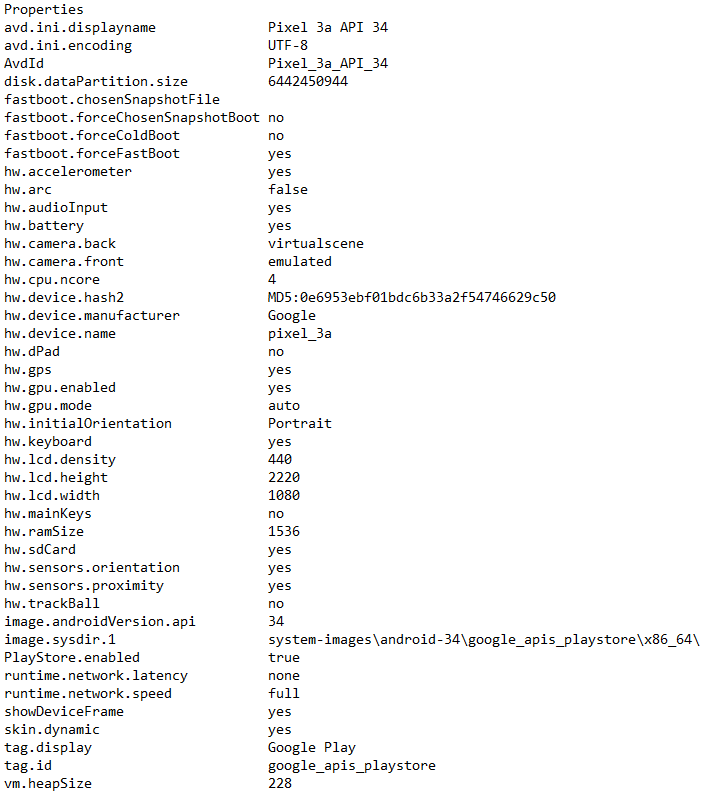
\includegraphics[width=0.8\textwidth]{images/android_emu_fb_1.png}
  \caption{Einstellungen des Android-Emulators von Florian Brändle Pixel 3a.}
\end{figure}

\begin{figure}[H]
  \centering
  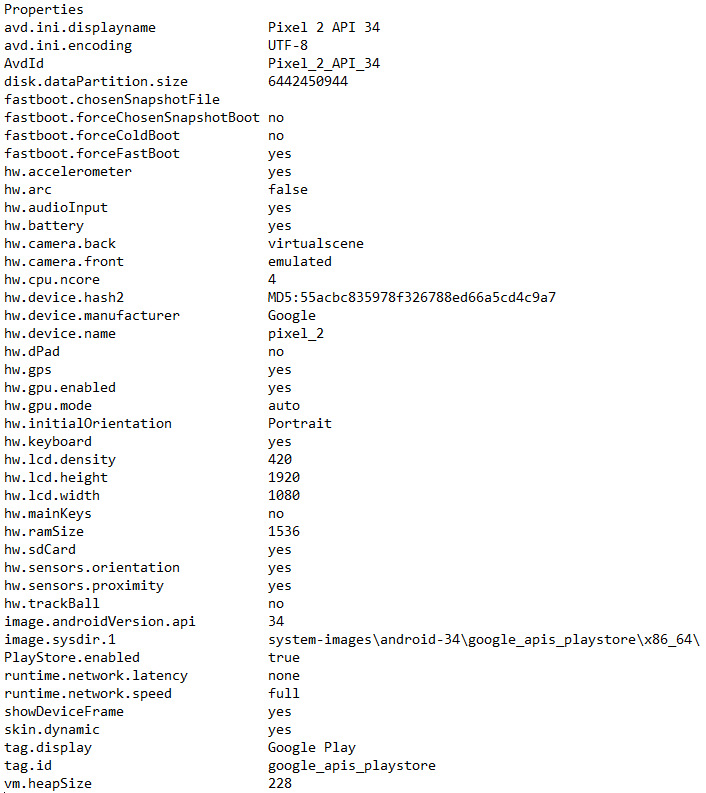
\includegraphics[width=0.8\textwidth]{images/android_emu_fb_2.png}
  \caption{Einstellungen des Android-Emulators von Florian Brändle Pixel 2.}
\end{figure}

\section{Hardware}

Die zwei Endgeräte auf denen getestet wurde, sind folgende:

\begin{itemize}
  \item iPhone 12 Pro, iOS 16.1.2 | IMEI: 35 861174 3743835
  \item Nokia 7 Plus, Android 10
\end{itemize}

